%! TEX root = ../../master.tex
\lecture[$k$-Zellen. CW-Komplexe. Realisierung von Sphären, Tori und  $\R\mathbb{P}^n$ als CW-Komplexe.]{Di 06 Jul 2021}[21]{CW-Komplexe}[Fortsetzung]

\section{CW-Komplexe}\label{sec:cw-komplexe}
\begin{definition}[$k$-Zelle]\label{def:k-zelle}
    Eine \vocab{$k$-Zelle},  $k\geq 0$, ist ein Raum der homöomorph zu $D^k$ ist. Eine \vocab{offene $k$-Zelle} ist eine ein Raum, der homöomorph zu ${D^k}\degree$  ist, wobei wie üblich
    \[
        D^k \coloneqq  \left \{(x,\ldots,x_k) \mid  \sum x_i ^2 \leq  1\right\} \\
        {D^k}\degree \coloneqq  \left \{(x_1,\ldots,x_k) \mid  \sum x_i^2 < 1\right\} 
    .\] 
    Wir nenen $k$ die  \vocab{Dimension} der Zelle. 
\end{definition}

\begin{definition}{CW-Komplex}\label{def:cw-komplex}
    Ein CW-Komplex  $X$ ist ein Hausdorff-Raum, der in offene Zellen  $\left \{c_i\right\} _{i \in I}$ zerfällt, wobei gilt:
    \begin{enumerate}[1.]
        \item Zu jeder $k$-Zelle  $c_i \subset X$ existiert eine stetige Abbildung $f_i \colon  D^k \to  X$, sodass ${D^k}\degree \subset D^k$ homöomorph auf $c_i$ und der Rand  $\partial D^k = S^{k-1} \subset D^k$ in eine Vereinigung von endlich vielen Zellen der Dimension $<k$ abgebildet wird. 
        \item $M\subset X$ ist genau dann offen, wenn $M \cap f_i(D^k)$ für alle $i\in I$ offen ist.
    \end{enumerate}
\end{definition}

\begin{oral}
    $C$ stet für 'closure finite', und  $W$ steht für 'weak'.
\end{oral}

\begin{dnotation}
    Das \vocab{k}-Gerüst oder auch \vocab{k}-Skelett von $X$, notiert  $X^k$, ist die Vereinigung aller seiner Zellen der Dimension  $\leq k$.  
\end{dnotation}

\begin{remark}
    Jeder CW-Komplex ist normal (und Hausdorff) sowie lokal zusammenziehbar, d.h. jeder Punkt besitzt eine zusammenziehbare Umgebung.

    Insbesondere ist jeder CW-Komplex
    \begin{itemize}
        \item lokal wegzusammenhängend
        \item (semi) lokal einfachzusammenhängend
    \end{itemize}
    und damit besitzt er eine universelle Überlagerung.
\end{remark}


\begin{question}
    Wie bildet man einen CW-Komplex?
\end{question}

Meistens erfolgt das mit einer induktiven / rekursiven Konstruktion, indem wir nacheinander die $k$-Skelette spezifizieren. Wir starten mit 
 \begin{enumerate}[1.]
     \item $X^0$, das  $0$-Gerüst, ist ein diskreter Raum (Punkte sind  $0$-Zellen).
     \item Haben wir das $k$-Gerüst $X^k$, $k\geq 0$ bereits gegebn, und eine Abbildung
         \[
         \varphi _{α}\colon  \partial D^{k+1} = S^k \longrightarrow  X^k
         .\] 
         so können wir eine $k+1$-Zelle an  $X^k$ 'ankleben'. Dazu betrachte
          \[
\faktor{X^k \bigsqcup D^{k+1}}{x \sim  \varphi _{α}(x)} =: X^k \cup_{\varphi _{α}} D^{k+1}
         .\] 
         so setzen wir
         \[
             X^{k+1} \coloneqq  X^k \cup _{\left \{\varphi _{α}\right\} } (D^{k+1})_{α}
         .\] 
         indem wir alle $k+1$-Zellen gleichzeitig ankleben.
\end{enumerate}

\begin{remark}
    Für endliche CW-Komplexe stimmen die Quotiententopologie und die schwache Topologie überein.
\end{remark}

\begin{oral}
    Für unendliche Räume erhalten wir genau die Kolimestopologie.
\end{oral}

\begin{oral}
    Der Hawaiianische Ohrring ist kein CW-Komplex.
\end{oral}

\begin{notation*}
    Ist $X$ ein CW-Komplex, und existiert  $N$, sodass  $X = X^N$ mit  $N$ minimal, so heißt  $N$ die  \vocab{Dimension} von $X$. 
\end{notation*}

\begin{example}
    Ein 1-dimensionaler CW-Komplex heißt auch \vocab{Graph}. Er besteht aus 0-Zellen und 1-Zellen. Die 0-Zellen nennen wir \vocab{Ecken} oder auch \vocab{Knoten}, die 1-Zellen \vocab{Kanten}.
\[
    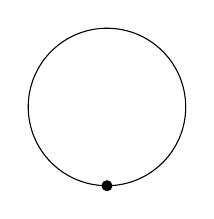
\begin{tikzpicture}
        \draw (0,0) circle (1);
        \fill (0,-1) circle (2pt);
    \end{tikzpicture}
\]
\missingfigure{Graph}
\begin{oral}
    \begin{warning}
        Man muss aufpassen, was passiert, wenn es unendlich viele Kanten in einem Punkt gib.
    \end{warning}
\end{oral}
\end{example}

\begin{example}[zwei-dimensional]
    Die Sphäre kann auch als CW-Komplex realisiert werden, indem wir eine 0-Zelle und eine 2-Zelle verwenden. Starten wir mit einem Punkt, so gibt es eine offensichtliche Abbildung $\partial D^2 \to  X^0 = \left \{S\right\} $. Wir kleben dann einfach den Rand von $D^2$ an den Punkt und erhalten sofort die Kugel.

    Alternativ kann man $S^n$ auch induktiv aufbauen, indem wir verwenden, dass  $S^n$ der Äquator von  $S^{n+1}$ ist, und dann jeweils 2 $n+1$-Zellen an  $S^n$ kleben, um  $S^{n+1}$ zu erhalten.

    Schauen wir nun auf $\R\mathbb{P}^n \coloneqq  \faktor{S^n}{x \sim -x}$, so sehen wir, dass wir die beiden Zellen, die wir für $S^n$ bekommen haben, jeweils identifizieren. Wir können  $\R\mathbb{P}^n$ also realisieren als CW-Komplex mit einer 0, einer 1, \ldots, und einer $n$-Zelle.

    Ein weiterer toller Punkt dieser auf den ersten Blick aufwendigeren Zellstruktur für  $S^n $ ist, dass wir nun
    \[
    S^{\infty} \coloneqq  \bigcup_{k=0}^{\infty} S^k 
    .\] 
    als die unendlich-dimensionale Sphäre als CW-Komplex definiert / realisiert haben.

    Der Torus kann ebenfalls so realisiert werden, hierzu benötigen wir eine 0-Zelle, zwei 1-Zellen sowie eine 2-Zelle.

    Erinnern wir uns an $\R\mathbb{P}^2 \coloneqq  \faktor{S^2}{x \sim  -x} \cong \faktor{D^2}{x \sim  -x \text{ für }x \in \partial D^2}$. Damit erhalten wir wieder eine Darstellung von $\R\mathbb{P}^2$ als eine 0, eine 1 und eine 2-Zelle.
\end{example}


\subsection{Berechnung der Fundamentalgruppe eines CW Komplexes}

\lecture[Berechunng der Fundamentalgruppe von Graphen]{Di 13 Jul 2021}[23]{Fundamentalgruppen von Graphen.}[Fortsetzung]

\begin{theorem}[Graphen]\label{thm:fundamentalgruppe-von-graphen}
    Sei $X$ ein wegzusammenhängender Graph, und  $x_0\in X^0$, d.h.
    \[
    X = \underbrace{\bigcup_{i \in  I^0} e_i^0 }_{X^0} \cup \underbrace{\bigcup_{i \in  I^1} e_i^1
}_{1-\text{Zellen}} 
    .\]
    Dann gilt:
    \begin{enumerate}[(i)]
        \item Es existiert $J\subset I^1$, so dass
            \[
            Y \coloneqq  X^0 \cup \bigcup_{j\in J} e_j^1
            .\] 
            ein maximaler \vocab{Baum} (ein zusammenziehbarer Graph, kombinatorisch: ein kreisfreier, zusammenhängender Graph) in $X$ ist. 
        \item Für $J$ wie in  $(i)$ gilt
             \[
                 \pi_1(X,x_0) \cong \coprod_{i\in I^1 \setminus J} \mathbb{Z} \cong \amalgprod_{i\in I^1 \setminus J} \mathbb{Z}
            .\] 
    \end{enumerate}
    Insbesondere ist die Fundamentalgruppe eines Graphen stets frei.
\end{theorem}

\begin{oral}
    Auch hier begnügen wir uns mit Beispielen, und führen keinen Beweis.
\end{oral}

\todo{TikZ von den Graph erstellen}
\begin{example}
    \begin{itemize}
        \item 
    Betrachte folgenden Graph:
    \missingfigure{Graph mit Baum}
    der grün markierte Teilgraph ist nun ein Baum. Für die Berechnung der Fundamentalgruppe ziehen wir nun den Baum zusammen, also erhalten wir noch:
    \[
       X \simeq Y \coloneqq 
       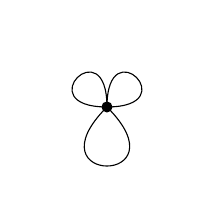
\begin{tikzpicture}[baseline = -0.2]
        \fill (0,0) circle (2pt);
        \draw (0,0) .. controls (1,0) and (0,1) .. (0,0);
        \draw (0,0) .. controls (0,1) and (-1,0) .. (0,0);
        \draw (0,0) .. controls (-1,-1) and (1,-1) .. (0,0);
    \end{tikzpicture}
\]
Der zusammengezogene Raum $Y$ ist dann tatsächlich homotop zum ursprünglichen Raum $X$, und  $Y$ ist nun frei mit so vielen Erzeugern, wie es Kanten in  $I^1 \setminus J$ gibt.
\item Betrachte  $Z$
    \[
    \begin{tikzcd}
        \arrow[loop left]{a} \ar{r}{b} x & y \ar[loop right]{c}
    \end{tikzcd}
\]
Dann ist $\pi_1(Z) = \left< α,β \mid  \right> $. Die Erzeuger sind gegeben durch $a, bcb^{-1}$
\item Ist $Z'$ der folgende Graph:
    \missingfigure{Graph}
    So sind die Erzeuger gegeben durch $a,bc b^{-1}, bd$
    \end{itemize}
\end{example}
